% $Id: template.tex 11 2007-04-03 22:25:53Z jpeltier $

%\documentclass{vgtc}                          % final (conference style)
%\documentclass[review]{vgtc}                 % review
%\documentclass[widereview]{vgtc}             % wide-spaced review
\documentclass[preprint]{vgtc}               % preprint
%\documentclass[electronic]{vgtc}             % electronic version

%% Uncomment one of the lines above depending on where your paper is
%% in the conference process. ``review'' and ``widereview'' are for review
%% submission, ``preprint'' is for pre-publication, and the final version
%% doesn't use a specific qualifier. Further, ``electronic'' includes
%% hyperreferences for more convenient online viewing.

%% Please use one of the ``review'' options in combination with the
%% assigned online id (see below) ONLY if your paper uses a double blind
% review process. Some conferences, like IEEE Vis and InfoVis, have NOT
%% in the past.

%% Figures should be in CMYK or Grey scale format, otherwise, colour 
%% shifting may occur during the printing process.

%% These few lines make a distinction between latex and pdflatex calls and they
%% bring in essential packages for graphics and font handling.
%% Note that due to the \DeclareGraphicsExtensions{} call it is no longer necessary
%% to provide the the path and extension of a graphics file:
%% \includegraphics{diamondrule} is completely sufficient.
%%
\ifpdf%                                % if we use pdflatex
  \pdfoutput=1\relax                   % create PDFs from pdfLaTeX
  \pdfcompresslevel=9                  % PDF Compression
  \pdfoptionpdfminorversion=7          % create PDF 1.7
  \ExecuteOptions{pdftex}
  \usepackage{graphicx}                % allow us to embed graphics files
  \DeclareGraphicsExtensions{.pdf,.png,.jpg,.jpeg} % for pdflatex we expect .pdf, .png, or .jpg files
\else%                                 % else we use pure latex
  \ExecuteOptions{dvips}
  \usepackage{graphicx}                % allow us to embed graphics files
  \DeclareGraphicsExtensions{.eps}     % for pure latex we expect eps files
\fi%

%% it is recomended to use ``\autoref{sec:bla}'' instead of ``Fig.~\ref{sec:bla}''
\graphicspath{{figures/}{pictures/}{images/}{./}} % where to search for the images
\usepackage{hyperref} 
\usepackage{microtype}                 % use micro-typography (slightly more compact, better to read)
\usepackage[OT1]{fontenc} 
\PassOptionsToPackage{warn}{textcomp}  % to address font issues with \textrightarrow
\usepackage{textcomp}                  % use better special symbols
\usepackage{mathptmx}                  % use matching math font
\usepackage{times}
\usepackage[english,ngerman]{babel}                     % we use Times as the main font
\renewcommand*\ttdefault{txtt}         % a nicer typewriter font
\usepackage{cite}                      % needed to automatically sort the references
\usepackage{tabu}                      % only used for the table example
\usepackage{booktabs}                  % only used for the table example
%% We encourage the use of mathptmx for consistent usage of times font
%% throughout the proceedings. However, if you encounter conflicts
%% with other math-related packages, you may want to disable it.


%% If you are submitting a paper to a conference for review with a double
%% blind reviewing process, please replace the value ``0'' below with your
%% OnlineID. Otherwise, you may safely leave it at ``0''.
\onlineid{0}

%% declare the category of your paper, only shown in review mode
\vgtccategory{Research}

%% allow for this line if you want the electronic option to work properly
\vgtcinsertpkg

%% In preprint mode you may define your own headline.
\preprinttext{Seminar Virtual und Augmented Reality -- WS 2019/20}

%% Paper title.

\title{Sensorisches Zusammenspiel des visuellen und vestibul\"aren Systems in Virtual Reality}


\author{Nils Henrik Seitz\thanks{e-mail: nils.seitz@uni-rostock.de}\\ %
        \scriptsize Universität Rostock }

%% A teaser figure can be included as follows, but is not recommended since
%% the space is now taken up by a full width abstract.
%\teaser{
%  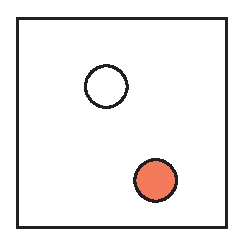
\includegraphics[width=1.5in]{sample.eps}
%  \caption{Lookit! Lookit!}
%}

%% Abstract section.
\abstract{
	Durch die zunehmende Digitalisierung der Gesellschaft, sinkende Kosten und gleichzeitig steigende Leistungsf\"ahigkeit der erfordlichen Hardware erfreut sich Virtual Reality immer gr\"oßerer Beliebtheit.

} % end of abstract

%% ACM Computing Classification System (CCS). 
%% See <http://www.acm.org/class/1998/> for details.
%% The ``\CCScat'' command takes four arguments.

\CCScatlist{ 
  \CCScat{H.1.2}{Models and Principles}%
	{User/Machine Systems}{Human factors, Human information processing};
  \CCScat{H.5.1}{Information Interfaces and Presentation (e.g., HCI)}%
	{Multimedia Information Systems}{Artificial, augmented, and virtual realities};
}

\keywords{Visual-vestibular conflict, motion sickness, cyber sickness, }

%% Copyright space is enabled by default as required by guidelines.
%% It is disabled by the 'review' option or via the following command:
% \nocopyrightspace

%%%%%%%%%%%%%%%%%%%%%%%%%%%%%%%%%%%%%%%%%%%%%%%%%%%%%%%%%%%%%%%%
%%%%%%%%%%%%%%%%%%%%%% START OF THE PAPER %%%%%%%%%%%%%%%%%%%%%%
%%%%%%%%%%%%%%%%%%%%%%%%%%%%%%%%%%%%%%%%%%%%%%%%%%%%%%%%%%%%%%%%%

\begin{document}

%% The ``\maketitle'' command must be the first command after the
%% ``\begin{document}'' command. It prepares and prints the title block.

%% the only exception to this rule is the \firstsection command
%% \firstsection{Einleitung}

\maketitle

\section{Einleitung} %for journal use above \firstsection{..} instead 
	Evolution\"ar gesehen, ist es die gr\"o{\ss}te St\"arke des Menschen, sich seiner Umgebung oder auch seine Umgebung an sich anzupassen. Daher liegt es in der Natur des Menschen, sich Werkzeuge herzustellen und Erfindungen zu machen, die im Alltag hilfreich sind.

Eine der wichtigsten Grundlagen daf\"ur ist die multisensorische Integration, ein evolution\"ares Wunder f\"ur sich, denn sie erm\"oglicht ein hohes, abstraktes Verst\"andnis und die F\"ahigkeit zu lernen. Unser Gehirn f\"uhrt unbemerkt und scheinbar m\"uhelos mehrmals innerhalb einer Sekunde die Informationen verschiedener Sinne zu einem f\"ur uns konsistenten Gesamtbild zusammen.
Dass diese Verarbeitung \"uberhaupt stattfindet, ist uns selten bewusst\cite{Deroy:2016:SensInte}. Sobald es dabei aber zu Komplikationen, das hei{\ss}t, Abweichungen der bisherigen Erfahrung, kommt, bemerken wir dies sofort. 

Eine relativ neue Erfindung ist Virtual Reality, mit der wir erstmalig die Chance haben, unsere Umgebung vollst\"andig nach unseren Vorstellung zu formen, beispielsweise auch mit ver\"anderten physikalischen Gesetzen.
Virtual Reality hat das enorme Potential, viele Bereiche der Gesellschaft nachhaltig zu ver\"andern, nur trifft es sich leider, dass genau bei der Integration der Sensorik Schwierigkeiten auftreten, die als Cyber Sickness bekannt sind.


\section{Methoden}
% Make Structure(section, sub(sub)sections, enumerate/itemize, figures and tables (see original for formatting (LABEL THEM, do captions, width and centering)), <- AUTOREF, make cites (FROM BIBDESK!!) and footnotes, sparsely use texttt / -it / -bf, use good latex style (symbols, equtions, etc.) and good indentation!)

%% FIGURES
%\begin{figure}[tb]
%	\centering % avoid the use of \begin{center}...\end{center} and use \centering instead (more compact)
%	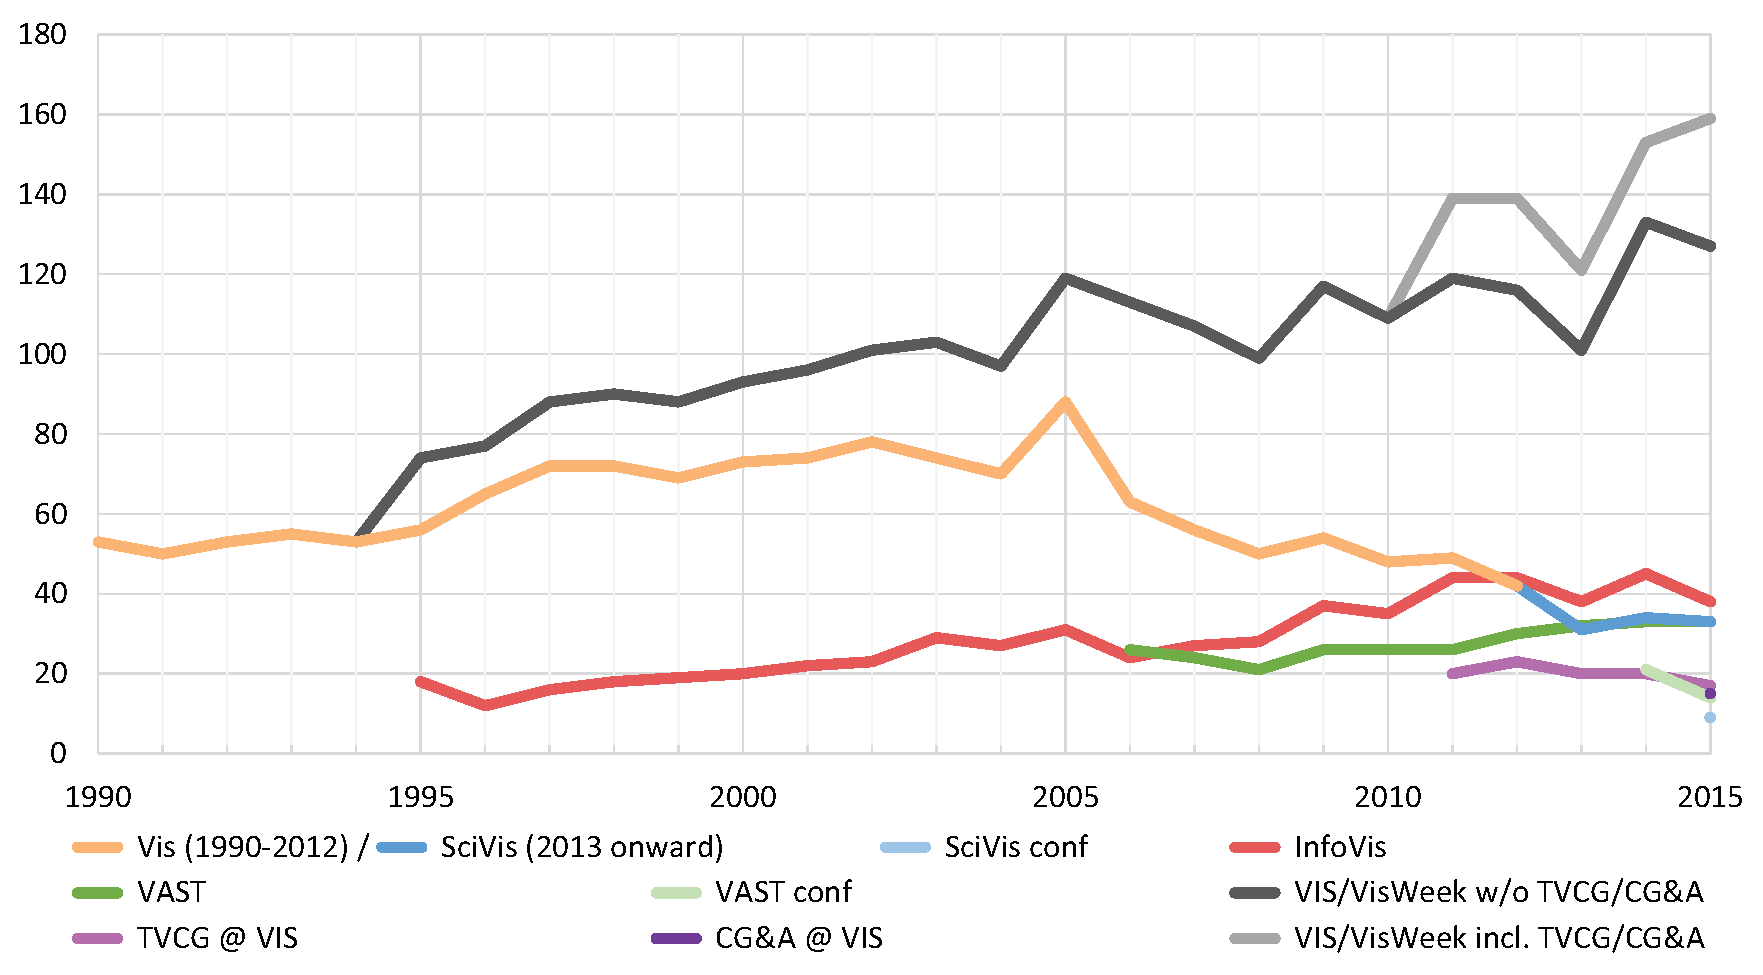
\includegraphics[width=\columnwidth]{paper-count-w-2015-new}
%	\caption{A visualization of the data from \autoref{tab:vis_papers}. The image is from \cite{Isenberg:2017:VMC} and is in the public domain.}
%	\label{fig:sample}
%\end{figure}
	test

\section{Ergebnisse}
	test

\section{Fazit}
	Cyber Sickness entsteht durch eine Form des visuell-vestibul\"aren Konflikts und ist, auf Grund der entstehenden Symptome, ein zentraler Aspekt der Nutzung von Virtual Reality. Diese k\"onnen das Erlebnis in einer virtuellen Realit\"at unertr\"aglich machen.

Es wurden in \autoref{Maßnahmen gegen CS} eine Reihe verschiedener Methoden vorgestellt, mit deren Hilfe man, vor allem durch Kombination der Methoden und unter Beachtung bestimmter Faktoren, Cyber Sickness reduzieren kann. Das generelle Prinzip der Nat\"urlichkeit oder Vertrautheit, das es einzuhalten gilt, zieht sich durch die Ma{\ss}nahmen.
Dieses Wissen kann helfen, in Zukunft einen besseren, f\"ur den Anwender angenehmeren Umgang mit weniger Cyber Sickness-Symptomen in Virtual Reality zu erm\"oglichen. Dennoch haben diese Methoden nur bedingte G\"ultigkeit und \"Ubertragbarkeit, da es sich hierbei noch um Grundlagenforschung handelt.

Es ist wichtig zu verstehen, dass momentan keine Theorie existiert, die die Ph\"anomene von Cyber Sickness vollst\"andig erkl\"aren kann. Daher ist es auch nicht m\"oglich zu sagen, ob Cyber Sickness und klassische Motion Sickness denselben Ursprung haben. Dennoch beziehen sich viele Studien \"uber Cyber Sickness in Virtual Reality auf \"altere Studien, in denen es eigentlich um klassische Motion Sickness oder Simulator Sickness geht und versuchen, \"ahnliche Ergebnisse im Sinne der Sensory Conflict Theory zu finden. Dies hat oft widerspr\"uchliche Ergebnisse zur Folge.

Weiterhin folgt aus dieser "`Vererbung"' von der klassischen Motion Sickness an die Cyber Sickness, dass in der Literatur keine eindeutige Nomenklatur herrscht, in der Begriffe wie Cyber Sickness, Virtual Reality Sickness, Simulator Sickness und Motion Sickness teils synonym verwendet werden, ohne dass dies gerechtfertig ist, da es keine genauen Definitionen f\"ur die jeweiligen Begriffe gibt.

Ausgehend von einer exakteren Benennung wird dann zus\"atzliche Forschung ben\"otigt, um eine bessere Theorie zur Erkl\"arung von Cyber Sickness zu finden. Auch m\"ussen neue Messverfahren erschlossen werden, da viele der Messung aktuell auf Selbstausk\"unften beruhen, welche subjektiv verf\"alscht sein k\"onnen. Durch Umsetzen dieser drei Punkte w\"urden danach eindeutigere, weniger widerspr\"uchliche und vor allem besser vergleichbare Ergebnisse entstehen. Es ist wichtig, dies nicht zu vernachl\"assigen, w\"ahrend in der Zwischenzeit mit den aktuellen Gegebenheiten weitergeforscht wird.

Zuletzt sollte bei zuk\"unftiger Forschung und der Umsetzung neuer Methoden an verschiedenste Gruppen gedacht werden, damit keine Ungleichheit zwischen Gruppen herrscht, wie das bei der Passform der Head-Mounted Displays in \autoref{abb:hmdfit} der Fall war. Der Mensch hat sich in seiner Evolution \"uber die Zeit schon an verschiedenste Gegebenheiten angepasst, somit ist anzunehmen, dass selbiges auch f\"ur Virtual Reality gilt. Bis dahin m\"ussen wir uns aber selbst bestm\"oglich unterst\"utzen, durch eben genannte Verbesserung und mit Methoden gegen Cyber Sickness, damit wir das gro{\ss}e Potential, welches Virtual Reality innewohnt, effektiv nutzen k\"onnen.




\acknowledgments{
Der Autor m\"ochte Amon Ties Uerckwitz f\"ur die Zusammenarbeit im Themengebiet ''Human Factors and Perception`` danken.}

%\bibliographystyle{abbrv}
%\bibliographystyle{abbrv-doi}
%\bibliographystyle{abbrv-doi-narrow}
%\bibliographystyle{abbrv-doi-hyperref}
\bibliographystyle{abbrv-doi-hyperref-narrow}

\bibliography{sources}
\end{document}
